\documentclass[answers]{exam}
\usepackage{texPreamble}
\usepackage{relsize}
\usepackage{tabularx}
\extraheadheight{0.25in}
\extrafootheight{1.0in}
\extrawidth{1in}
% ----------------------------------------------------------------

\begin{document}
%\relscale{1.4}
    \section{JIT 4.7: Intersection of curves and simultaneous solutions}
    \begin{ex*}\ 
    
      $\begin{array}{l}
        y=x^2-4\\
        x+y=8
      \end{array}$
      \vspace*{\stretch{1}}
    \end{ex*}
    
    \pagebreak

    \begin{ex*}\ 
    
      $\begin{array}{r@{\,=\,}l}
        2x+3y&7\\
        -3x+7y&11
      \end{array}$
    \end{ex*}
    
    \vspace*{\stretch{1}}
    \begin{minipage}[t]{0.5\linewidth}
    \noindent
    \begin{ex*}\ 
    \end{ex*}
      $\begin{array}{r@{\,=\,}l}
        y&x+7\\
        y&(x-2)^2+3
      \end{array}$
    \end{minipage}%
    \begin{minipage}[t]{0.5\linewidth}\ 
      \begin{center}
          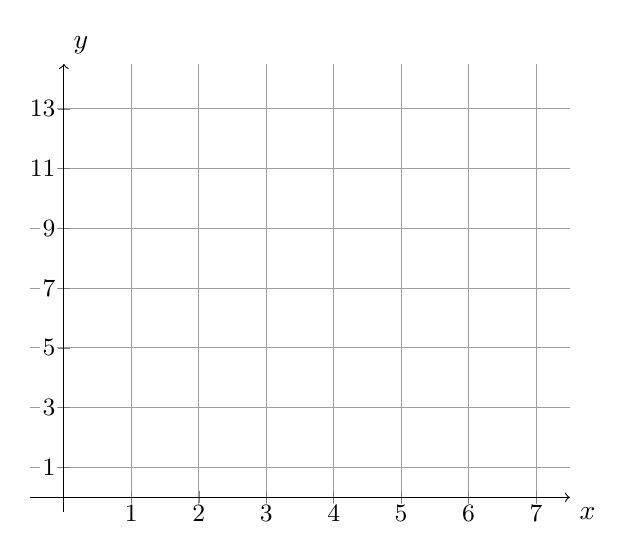
\begin{tikzpicture}[scale=1.0]
            \begin{axis}[
              axis lines=center,
              axis line style={->},
              grid=both,
              grid style={line width=0.35pt, draw=gray!75},
              xmin=-0.5, xmax=7.5,
              ymin=-0.5, ymax=14.5,
              xtick={-4,-3,...,7},
              ytick={-3,-1,...,14},
              ticklabel style={font=\small, inner sep=0.75pt, fill=white},
              xlabel=$x$, xlabel style={at={(ticklabel* cs:1)},anchor=north west},
              ylabel=$y$, ylabel style={at={(ticklabel* cs:1)},anchor=south west},
              ]
              
            \end{axis}
          \end{tikzpicture}
        \end{center}
    \end{minipage}

  \pagebreak
\end{document}
